% SIAM Article Template
\documentclass[review]{siamart0216}

\usepackage[utf8]{inputenc}

\usepackage{hyperref}
\usepackage{graphicx}
\usepackage{amsmath}
\usepackage{caption}
\graphicspath{ {images/} }

\usepackage{upquote}

\usepackage{amsmath}
\usepackage{url}
\usepackage{hyperref}

% this is required for all the \url{} commands in the bib file
%\usepackage{hyperref}

% for nice units
\usepackage{siunitx}

% for images: png, pdf, etc
\usepackage{graphicx}

% for nice table formatting, i.e., /toprule, /midrule, etc
\usepackage{booktabs}

% to allow for \verb++ declarations in captions.
\usepackage{cprotect}

% to allow usage of \mathbb symbols
\usepackage{amssymb}

\usepackage{longtable}

\title{SymPy: Symbolic Computing in Python}

\input{authors}

\begin{document}
\maketitle

\section{Introduction}

%% What sympy is, where to download etc.
%%
%% List other major CASs.
%%
%% Why SymPy.

SymPy is a full featured computer algebra system (CAS) written in the Python
programming language. It is open source, being licensed under the extremely
permissive 3-clause BSD license.
% cite BSD?
SymPy was started by Ond\v{r}ej \v{C}ert\'{\i}k in 2005, and it has since
grown into a large open source project, with over 500 contributors. SymPy is
developed on GitHub using a bazaar community
model~\cite{raymond1999cathedral}. The accessibility of the codebase and the
open community model allows SymPy to rapidly respond to the needs of the
community of users, and has made the large contributor count possible.
% citation?

SymPy is written entirely in the Python programming language.
% cite Python?
Python is a popular dynamically typed programming language that has a focus on
ease of use and readability. It also a very popular language for scientific
computing and data science, with a wide range of useful
libraries~\cite{oliphant2007python}. SymPy is itself used by many libraries
and tools across many domains, such as Sage~\cite{SAGE} (pure mathematics),
yt~\cite{2011ApJS..192....9T} (astronomy and astrophysics),
PyDy~\cite{gede2013constrained} (multibody dynamics), and
SfePy~\cite{cimrman2014sfepy} (finite elements).

Unlike many CASs, SymPy does not invent its own programming language. Python
is used both for the internal implementation and the user interaction.
Exclusively using Python in this way makes it easier for people already
familiar with the language to use or develop SymPy. It also lets the SymPy
developers focus on mathematics, rather than language design.

SymPy is designed with a strong focus that it be usable as a library. This
means that extensibility is important in its application program interface
(API) design. This is also one of the reasons SymPy makes no attempt to extend
the Python language itself. The goal is for users of SymPy to be able to
import SymPy alongside other Python libraries in their workflow, whether that
is an interactive workflow or programmatic use as part of a larger system.

Being developed as a library, SymPy does not have a built-in graphical user
interface (GUI). However, SymPy exposes a rich interactive display system,
including registering printers with Jupyter~\cite{perez2007ipython} frontends,
including the Notebook and Qt Console, which will pretty print SymPy
expressions using MathJax~\cite{cervone2012mathjax} or \LaTeX{} rendering.

Section~\ref{sec:architecture} discusses the architecture of SymPy. Following
that, Section~\ref{sec:numerics} looks at the numerical features of SymPy and
its dependency library, mpmath. Section~\ref{sec:features} enumerates the
features of SymPy and takes a closer look at some of the important ones.
Section~\ref{sec:domain_specific} looks at the domain specific physics
submodules for doing classical mechanics and quantum mechanics. Finally,
Section~\ref{sec:conclusion} concludes the paper and discusses future work.


\section{Architecture}

\subsection{Basic Usage}

% symbols, various ways to declare them

Being built on Python, SymPy requires that all variable names be defined
before they can be used. The statement
\begin{verbatim}
>>> from sympy import *
\end{verbatim}
will import all SymPy functions into the global Python namespace. All the
examples in this paper assume that this has been run.

Symbolic variables, called symbols, must be defined and assigned to
Python variables before they can be used. This is typically done through the
\texttt{symbols} function, which creates multiple symbols at once. For
instance,
\begin{verbatim}
>>> x, y, z = symbols('x y z')
\end{verbatim}
creates three symbols representing variables named $x$, $y$, and $z$, assigned
to Python variables of the same name. The Python variable names that symbols
are assigned to are immaterial---we could have just as well have written
\verb|a, b, c = symbol('x y z')|. All the examples in this paper will assume
that the symbols \verb|x|, \verb|y|, and \verb|z| have been assigned as above.

Expressions are created from symbols using Python syntax, which mirrors usual
mathematical notation. Note that in Python, exponentiation is \verb|**|. For
instance, the following creates the expresion $(x^2 - 2x + 3)/y$.
\begin{verbatim}
>>> (x**2 - 2*x + 3)/y
(x**2 - 2*x + 3)/y
\end{verbatim}

All SymPy expressions are immutable. This simplifies the design by allowing
interning. It also allows expressions to be hashed and stored in a Python
dictionary, which enables caching and other features.

%% I volunteer to write this section. --Aaron
%%
%% Representing symbolic expressions using Python objects

\subsection{The Core}

The core of a computer algebra system (CAS) refers to the module that is in
charge of representing symbolic expressions and performing basic manipulations
with them. In SymPy, every symbolic expression is an instance of a Python class.
Expressions are represented by expression trees. The operators are represented
by the type of an expression and the child nodes are stored in the
\texttt{args} attribute. A leaf node in the expression tree has an empty
\texttt{args}.
The \texttt{args} attribute is provided by the class \texttt{Basic},
which is a superclass of all SymPy objects and
provides common methods to all SymPy tree-elements.
For example, consider the expression $xy + 2$:
\begin{verbatim}
>>> expr = x*y + 2
\end{verbatim}
By order of operations, the parent of the expression tree for \texttt{expr} is
an addition, so it is of type \texttt{Add}. The child nodes of \texttt{expr} are
\texttt{2} and \texttt{x*y}.
\begin{verbatim}
>>> type(expr)
<class 'sympy.core.add.Add'>
>>> expr.args
(2, x*y)
\end{verbatim}

One can dig further into the expression tree to see the full expression. For
example, the first child node, given by \texttt{expr.args[0]} is
\texttt{2}. Its class is \texttt{Integer}, and it has empty \texttt{args},
indicating that it is a leaf node.
\begin{verbatim}
>>> expr.args[0]
2
>>> type(expr.args[0])
<class 'sympy.core.numbers.Integer'>
>>> expr.args[0].args
()
\end{verbatim}

A useful way to view an expression tree is with the \texttt{srepr} function,
which returns a string representation of an expression as valid Python code
with all the nested class constructor calls to create the given expression.
\begin{verbatim}
>>> srepr(expr)
"Add(Mul(Symbol('x'), Symbol('y')), Integer(2))"
\end{verbatim}

Every SymPy expression satisfies a key invariant, namely,
\verb|expr.func(*expr.args) == expr|. This means that expressions are
rebuildable from their \texttt{args}~\footnote{\texttt{expr.func} is used
instead of \texttt{type(expr)} to allow the function of an expression to be
distinct from its actual Python class. In most cases the two are the same.}.
Here, we note that in SymPy, the \texttt{==} operator represents exact
structural equality, not mathematical equality. This allows one to test if
any two expressions are equal to one another as expression trees.

Python allows classes to override mathematical operators. The Python
interpreter translates the above \texttt{x*y + 2} to, roughly,
\verb|(x.__mul__(y)).__add__(2)|. Both \texttt{x} and \texttt{y}, returned
from the \texttt{symbols} function, are \texttt{Symbol} instances. The
\texttt{2} in the expression is processed by Python as a literal, and is
stored as Python's builtin \texttt{int} type. When \texttt{2} is passed to the
\verb|__add__| method of \texttt{Symbol}, it is converted to the SymPy type
\verb|Integer(2)| before being stored in the resulting expression tree. In
this way, SymPy expressions can be built in the natural way using Python
operators and numeric literals.

One must be careful in one particular instance: Python does not have a builtin
rational literal type. Given a fraction of integers such as \texttt{1/2},
Python will perform floating point division and produce
\texttt{0.5}~\footnote{This is the behavior in Python 3. In Python 2,
  \texttt{1/2} will perform integer division and produce \texttt{0}, unless
  one uses \texttt{from \_\_future\_\_ import division}.}. Python uses eager
evaluation, so expressions like \texttt{x + 1/2} will produce \texttt{x +
  0.5}, because by the time any SymPy function sees the \texttt{1/2} it will
have already been converted to \texttt{0.5} by Python. However, for a CAS like
SymPy, one typically wants to work with exact rational numbers whenever
possible. Working around this is simple, however: one can wrap one of the
integers with \texttt{Integer}, like \verb|x + Integer(1)/2|, or using
\verb|x + Rational(1, 2)|. SymPy provides a function \texttt{S} which can be
used to convert objects to SymPy types with minimal typing, such as
\verb|x + S(1)/2|. This gotcha is a small downside to using Python directly
instead of a custom domain specific language (DSL), and we consider it to be
worth it for the advantages of using Python.

%%
%% Assumptions
\subsection{Assumptions}

An important feature of the SymPy core is the assumptions system. The
assumptions system allows users to specify that symbols have certain common
mathematical properties, such as being positive, imaginary, or integral. SymPy
is careful to never perform simplifications on an expression unless the
assumptions allow them. For instance, the identity $\sqrt{t^2} = t$ holds if
$t$ is nonnegative ($t\ge 0$). If $t$ is real, the identity $\sqrt{t^2}=|t|$
holds. However, for general complex $t$, no such identity holds.

By default, SymPy performs all calculations assuming that symbols are
complex valued. This assumption makes it easier to treat mathematical problems
in full generality.
\begin{verbatim}
>>> t = Symbol('t')
>>> sqrt(t**2)
sqrt(t**2)
\end{verbatim}

By assuming the most general case, that symbols are complex by default, SymPy
avoids performing mathematically invalid operations. However, in many cases
users will wish to simplify expressions containing terms like $\sqrt{t^2}$.

Assumptions are set on \texttt{Symbol} objects when they are created. For
instance \verb|Symbol('t', positive=True)| will create a symbol named
\texttt{t} that is assumed to be positive.
\begin{verbatim}
>>> t = Symbol('t', positive=True)
>>> sqrt(t**2)
t
\end{verbatim}
Some of the common assumptions that SymPy allows are \texttt{positive},
\texttt{negative}, \texttt{real}, \texttt{nonpositive}, \texttt{nonnegative},
\texttt{real}, \texttt{integer}, and \texttt{commutative}~\footnote{If $A$ and
$B$ are Symbols created with \texttt{commutative=False} then SymPy will keep
$A\cdot B$ and $B\cdot A$ distinct.}. Assumptions on any object can be checked with the
\verb|is_|\texttt{\textit{assumption}} attributes, like \verb|t.is_positive|.

Assumptions are only needed to restrict a domain so that certain
simplifications can be performed. It is not required to make the domain match
the input of a function. For instance, one can create the object
$\sum_{n=0}^m f(n)$ as \verb|Sum(f(n), (n, 0, m))| without setting
\texttt{integer=True} when creating the Symbol object \texttt{n}.

The assumptions system additionally has deductive capabilities. The
assumptions use a three-valued logic using the Python builtin objects
\texttt{True}, \texttt{False}, and \texttt{None}. \texttt{None} represents the
``unknown'' case. This could mean that the given assumption could be either
true or false under the given information, for instance,
\verb|Symbol('x', real=True).is_positive| will give \texttt{None} because a real
symbol might be positive or it might not. It could also mean not enough is
implemented to compute the given fact. For instance,
\verb|(pi + E).is_irrational| gives \texttt{None}, because SymPy does not know
how to determine if $\pi + e$ is rational or irrational, indeed, it is an open
problem in mathematics.
% TODO: ref?


Basic implications between the facts are used to deduce assumptions. For
instance, the assumptions system knows that being an integer implies being
rational, so \verb|Symbol('x', integer=True).is_rational| returns
\texttt{True}. Furthermore, expressions compute the assumptions on themselves
based on the assumptions of their arguments. For instance, if \texttt{x} and
\texttt{y} are both created with \texttt{positive=True}, then
\verb|(x + y).is_positive| will be \texttt{True}.

SymPy also has an experimental assumptions system where facts are stored
separate from objects, and deductions are made with a SAT solver. We will not
discuss this system here.

%%
%% Extensibility
\subsection{Extensibility}

Extensibility is an important feature for SymPy. Because the same language,
Python, is used both for the internal implementation and the external usage by
users, all the extensibility capabilities available to users are also used by
functions that are part of SymPy.

The typical way to create a custom SymPy object is to subclass an existing
SymPy class, generally either \texttt{Basic}, \texttt{Expr}, or
\texttt{Function}. All SymPy classes used for expression trees~\footnote{Some
  internal classes, such as those used in the polynomial module, do not follow
  this rule for efficiency reasons.} should be subclasses of the base class
\texttt{Basic}, which defines some basic methods for symbolic expression
trees. \texttt{Expr} is the subclass for mathematical expressions that can be
added and multiplied together. Instances of \texttt{Expr} typically represent
complex numbers, but may also include other ``rings'' like matrix expressions.
Not all SymPy classes are subclasses of \texttt{Expr}. For instance, logic expressions, such
as \verb|And(x, y)| are subclasses of \texttt{Basic} but not of \texttt{Expr}.

The \texttt{Function} class is a subclass of \texttt{Expr} which makes it
easier to define mathematical functions called with arguments. This includes
named functions like $\sin(x)$ and $\log(x)$ as well as undefined functions
like $f(x)$. Subclasses of \texttt{Function} should define a
class method \texttt{eval}, which returns values for which the function should
be automatically evaluated, and \texttt{None} for arguments that should not be
automatically evaluated.

Many SymPy functions require various evaluations down the expression tree.  The
evaluation of such functions on of classes in SymPy is performed by defining a
relevant \verb|_eval_|\texttt{\textit{*}} method on the class. For instance, an
object can signal to SymPy's \texttt{diff} function how to take the derivative of
itself by defining the \verb|_eval_derivative(self, x)| method, which may in
turn call \texttt{diff} on its \texttt{args}. The most common
\verb|_eval_|\texttt{\textit{*}} methods relate to the assumptions.
\verb|_eval_is_|\texttt{\textit{assumption}} defines the assumptions for
\textit{assumption}.

As an example of the notions presented in this section, we present below
a stripped down version of the gamma function $\Gamma(x)$ from SymPy,
which evaluates itself on positive integer arguments, has the positive and
real assumptions defined, can be rewritten in terms of factorial with
\verb|gamma(x).rewrite(factorial)|, and can be differentiated.
\texttt{fdiff} is a convenience method for subclasses of \texttt{Function}.
\texttt{fdiff} returns the derivative of the function without worrying about
the chain rule. \texttt{self.func} is used throughout instead of referencing
\texttt{gamma} explicitly so that potential subclasses of \texttt{gamma} can
reuse the methods.
\begin{verbatim}
from sympy import Integer, Function, floor, factorial, polygamma

class gamma(Function)
    @classmethod
    def eval(cls, arg):
        if isinstance(arg, Integer) and arg.is_positive:
            return factorial(arg - 1)

    def _eval_is_real(self):
        x = self.args[0]
        # noninteger means real and not integer
        if x.is_positive or x.is_noninteger:
            return True

    def _eval_is_positive(self):
        x = self.args[0]
        if x.is_positive:
            return True
        elif x.is_noninteger:
            return floor(x).is_even

    def _eval_rewrite_as_factorial(self, z):
        return factorial(z - 1)

    def fdiff(self, argindex=1):
        from sympy.core.function import ArgumentIndexError
        if argindex == 1:
            return self.func(self.args[0])*polygamma(0, self.args[0])
        else:
            raise ArgumentIndexError(self, argindex)
\end{verbatim}
The actual gamma function defined in SymPy has many more capabilities, such as
evaluation at rational points and series expansion.


\section{Numerics}

%% Description of some algorithms (example: integration with Risch, Meijer G, Gruntz, polys)
%%
%% Description of numerics/mpmath (Fredrik)

The \texttt{Float} class holds an arbitrary-precision binary floating-point value
and a precision in bits. An operation between two \texttt{Float}
inputs is rounded to the larger of the two precisions.
Since Python floating-point literals automatically evaluate to \texttt{double}
(53-bit) precision, strings should be used to input precise decimal values:

\begin{verbatim}
>>> Float(1.1)
1.10000000000000
>>> Float(1.1, 30)   # precision equivalent to 30 digits
1.10000000000000008881784197001
>>> Float("1.1", 30)
1.10000000000000000000000000000
\end{verbatim}

The preferred way to evaluate an expression numerically is with the
\texttt{evalf} method, which internally estimates the number of accurate
bits of the floating-point
approximation for each sub-expression, and adaptively increases the
working precision until the estimated accuracy of the
final result matches the sought number of decimal digits.

The internal error tracking does not provide rigorous error bounds
(in the sense of interval arithmetic) and cannot be used to track
uncertainty in measurement data in any meaningful way;
the sole purpose is to mitigate loss of accuracy that typically occurs
when converting symbolic expressions to numerical values, for example
due to catastrophic cancellation. This is illustrated by the following
example (the input 25 specifies that 25 digits are sought):

\begin{verbatim}
>>> cos(exp(-100)).evalf(25) - 1
0
>>> (cos(exp(-100)) - 1).evalf(25)
-6.919482633683687653243407e-88
\end{verbatim}

The \texttt{evalf} method works with complex numbers and supports
more complicated expressions, such as
special functions, infinite series and integrals.

SymPy does not track the accuracy of
approximate numbers outside of \texttt{evalf}.
The familiar dangers of floating-point arithmetic apply~\cite{goldberg1991every}, and
symbolic expressions containing floating-point numbers should be treated
with some caution.
This approach is similar to Maple and Maxima.

By contrast, Mathematica uses a form
of significance arithmetic~\cite{Sofroniou2005precise} for approximate numbers.
This offers further protection against numerical errors,
but leads to non-obvious semantics while
still not being mathematically rigorous
(for a critique of significance arithmetic, see Fateman~\cite{Fateman1992}).
SymPy's \texttt{evalf} internals are non-rigorous in the same sense,
but have no bearing on the semantics of floating-point
numbers in the rest of the system.

\subsection{The mpmath library}

The implementation of arbitrary-precision floating-point arithmetic is
supplied by the mpmath library, which originally was developed as a SymPy
module but subsequently has been moved to a standalone pure Python package.
The basic datatypes in mpmath are \texttt{mpf} and \texttt{mpc}, which
respectively act as multiprecision substitutes for Python's \texttt{float} and
\texttt{complex}. The floating-point precision is controlled by a global
context:

% doctest printer doesn't display "mpf"
% no-doctest
\begin{verbatim}
>>> import mpmath
>>> mpmath.mp.dps = 30    # 30 digits of precision
>>> mpmath.mpf("0.1") + mpmath.exp(-50)
mpf('0.100000000000000000000192874984794')
>>> print(_)   # pretty-printed
0.100000000000000000000192874985
\end{verbatim}

For pure numerical computing, it is convenient to use mpmath directly
with \texttt{from mpmath import *} (it is best to avoid such an
import statement when using SymPy simultaneously, since numerical
functions such as \texttt{exp} will shadow the symbolic counterparts
in SymPy).

Like SymPy, mpmath is a pure Python library.
Internally, mpmath represents a floating-point number
${(-1)}^s x \cdot 2^y$ by a tuple $(s, x, y, b)$ where
$x$ and $y$ are arbitrary-size Python integers
and the redundant integer $b$ stores the bit length of $x$ for quick access.
If GMPY~\cite{GMPY} is installed, mpmath automatically switches to
using the \texttt{gmpy.mpz} type for $x$ and using GMPY helper methods
to perform rounding-related operations, improving performance.

The mpmath library includes support for
special functions, root-finding, linear algebra, polynomial approximation,
and numerical computation of limits, derivatives, integrals, infinite
series, and ODE solutions. All features work in arbitrary precision
and use algorithms that support computing hundreds of digits rapidly,
except in degenerate cases.

The double exponential (tanh-sinh) quadrature is used for numerical
integration by default. For smooth integrands, this algorithm usually
converges extremely rapidly, even when the integration interval is infinite
or singularities are present at the endpoints~\cite{takahasi1974double,bailey2005comparison}.
However, for good performance, singularities
in the middle of the interval must be specified
by the user.
To evaluate slowly converging limits and infinite series, mpmath
automatically attempts to apply Richardson extrapolation and the
Shanks transformation
(Euler-Maclaurin summation can also be used)~\cite{BenderOrszag1999}.
A function to evaluate oscillatory integrals by means of convergence
acceleration is also available.

A wide array of higher mathematical functions are implemented
with full support for complex values of all parameters and arguments,
including complete and incomplete gamma functions,
Bessel functions, orthogonal polynomials, elliptic functions and integrals,
zeta and polylogarithm functions,
the generalized hypergeometric function, and the Meijer G-function.

Most special functions are implemented as linear
combinations of the generalized hypergeometric function ${}_{p}F_{q}$,
which is computed by a combination of direct summation,
argument transformations (for ${}_2F_1$, ${}_3F_2$, $\ldots$)
and asymptotic expansions
(for ${}_0F_1$, ${}_1F_1$, ${}_1F_2$, ${}_2F_2$, ${}_2F_3$)
to cover the whole complex domain.
Numerical integration and generic convergence acceleration
are also used in a few special cases.

In general, linear combinations and argument transformations
give rise to singularities that have to be removed for certain
combinations of parameters.
A typical example is the modified Bessel function of the second kind

$$K_{\nu}(z) = \frac{1}{2} \left[
            {\left(\frac{z}{2}\right)}^{-\nu}
                \Gamma(\nu)
                {}_0F_1\!\left(1-\nu, \frac{z^2}{4}\right)
             -
             {\left(\frac{z}{2}\right)}^{\nu}
                 \frac{\pi}{\nu \sin(\pi \nu) \Gamma(\nu)}
                 {}_0F_1\!\left(\nu+1, \frac{z^2}{4}\right)
            \right]$$
where the limiting value $\lim_{\varepsilon \to 0} K_{n+\varepsilon}(z)$
has to be computed when $\nu = n$ is an integer.
A generic algorithm is used to evaluate
hypergeometric-type linear combinations of the above type.
This algorithm automatically detects cancellation problems,
and computes limits numerically by perturbing parameters whenever
internal singularities occur (the perturbation size is automatically
decreased until the result is detected to converge numerically).

Due to this generic approach, particular combinations of hypergeometric
functions can be specified easily.
The implementation of the Meijer G-function takes only a few dozen lines of
code, yet covers the whole input domain in a robust way.
The Meijer G-function instance
$G_{1, 3}^{3, 0}\left(0 ; \tfrac{1}{2}, -1, - \tfrac{3}{2} | x \right)$
is a good test case~\cite{Toth2007}; past versions of both Maple and
Mathematica produced incorrect numerical values for large $x > 0$.
Here, mpmath automatically removes the internal singularity
and compensates for cancellations (amounting to 656 bits
of precision when $x = 10000$), giving correct values:
\begin{verbatim}
>>> mpmath.mp.dps = 15
>>> mpmath.meijerg([[],[0]],[[-0.5,-1,-1.5],[]],10000)
2.4392576907199564e-94
\end{verbatim}

Equivalently, with SymPy's interface this function can be evaluated as:
\begin{verbatim}
>>> meijerg([[],[0]],[[-S(1)/2,-1,-S(3)/2],[]],10000).evalf()
2.43925769071996e-94
\end{verbatim}

We highlight the generalized hypergeometric functions and the Meijer
G-function, due to those functions' frequent appearance in closed forms for
integrals and sums (see Section~\ref{sec:calculus}). Via mpmath, SymPy has
relatively good support for evaluating sums and integrals numerically, using
two complementary approaches: direct numerical evaluation, or first computing
a symbolic closed form involving special functions.
% TODO: example?

\subsection{Numerical simplification}

The \texttt{nsimplify} function in SymPy
(a wrapper of \texttt{identify} in mpmath)
attempts to find a simple symbolic
expression that evaluates to the same numerical value as the given
input.
It works by applying a few simple transformations
(including square roots, reciprocals, logarithms and exponentials) to
the input and, for each transformed value,
using the PSLQ algorithm~\cite{Ferguson1999} to search for
a matching algebraic number or optionally a linear combination
of user-provided base constants (such as $\pi$).

\begin{verbatim}
>>> t = 1 / (sin(pi/5)+sin(2*pi/5)+sin(3*pi/5)+sin(4*pi/5))**2
>>> nsimplify(t)
-2*sqrt(5)/5 + 1
>>> nsimplify(pi, tolerance=0.01)
22/7
>>> nsimplify(1.783919626661888, [pi], tolerance=1e-12)
pi/(-1/3 + 2*pi/3)
\end{verbatim}


\section{Features}

%% List of Features and how to use
%%
%% Quick overview of the main modules, what it can do and so on. It should probably provide examples how to use sympy.
%%
%% See also the supplement (below)

% Features to discuss in-depth:

SymPy has an extensive feature set that encompasses too much to cover
in-depth here. Bedrock areas, such as calculus, receive their own sub-sections
below. Additionally, Table~\ref{features-table} describes other capabilities
present in the SymPy code base. This gives a sampling from the breadth of
topics and application domains that SymPy services.


\begin{longtable}[htbc]{p{0.25\linewidth}p{0.68\linewidth}}
\caption{SymPy Features and Descriptions\label{features-table}}\\
\toprule
\textbf{Feature} & \textbf{Description} \\
\midrule
Discrete Math & Summations, products, binomial coefficients,
    prime number tools, integer factorization, Diophantine equation solving, and
    boolean logic representation, equivalence testing, and inference.\\
Concrete Math & Tools for determining whether summation and product
    expressions are convergent, absolutely convergent, hypergeometric, and
    other properties. May also compute Gosper's normal form~\cite{petkovvsek1996bak} for two univariate polynomials.\\
Plotting & Hooks for visualizing expressions via matplotlib~\cite{Hunter:2007}
    or as text drawings when lacking a graphical back-end.\\
Geometry & Allows the creation of 2D geometrical entities,
    such as lines and circles. Enables queries on these entities, including
    asking the area of an ellipse, checking for collinearity of a set of
    points, or finding the intersection between two lines.\\
Statistics & Support for a random variable type as well as the ability to
    declare this variable from prebuilt distribution functions such as
    Normal, Exponential, Coin, Die, and other custom distributions.\\
Polynomials & Computes polynomial algebras over various coefficient domains
    ranging from the simple (e.g., polynomial division) to the advanced
    (e.g., Gr\"obner bases~\cite{adams1994introduction} and multivariate
    factorization over algebraic number domains).\\
Sets & Representations of empty, finite, and infinite sets. This includes
    special sets such as for all natural, integer, and complex numbers.\\
Series & Implements series expansion, sequences, and limit of sequences.
    This includes special series, such as Fourier and power series.\\
Vectors & Provides basic vector math and differential calculus with respect
    to 3D Cartesian coordinate systems.\\
Matrices & Tools for creating matrices of symbols and expressions.
    This is capable of both sparse and dense representations and performing
    symbolic linear algebraic operations (e.g., inversion and factorization).\\
Combinatorics \& Group Theory & Implements permutations, combinations,
    partitions, subsets,
    various permutation groups (such as polyhedral, Rubik, symmetric,
    and others), Gray codes~\cite{Nijenhuis1978combinatorial},
    and Prufer sequences~\cite{biggs1976graph}.\\
Code Generation & Enables generation of compilable and executable
    code in a variety of different programming languages directly from
    expressions. Target languages include C, Fortran, Julia, JavaScript,
    Mathematica, Matlab and Octave, Python, and Theano.\\
Tensors & Symbolic manipulation of indexed objects.\\
Lie Algebras & Represents Lie algebras and root systems.\\
Cryptography & Represents block and stream ciphers, including
    shift, Affine, substitution, Vigenere's, Hill's, bifid, RSA, Kid RSA,
    linear-feedback shift registers, and Elgamal encryption\\
Special Functions & Implements a number of well known special functions,
    including Dirac delta, Gamma, Beta, Gauss error functions, Fresnel
    integrals, Exponential integrals, Logarithmic integrals, Trigonometric
    integrals, Bessel, Hankel, Airy, B-spline, Riemann Zeta, Dirichlet eta,
    polylogarithm, Lerch transcendent, hypergeometric, elliptic integrals,
    Mathieu, Jacobi polynomials, Gegenbauer polynomial, Chebyshev polynomial,
    Legendre polynomial, Hermite polynomial, Laguerre polynomial, and
    spherical harmonic functions.\\
\bottomrule

\end{longtable}

\subsection{Simplification}

% polynomial expressions

% functions

% expand( ), factor( ), collect( ), together( ), apart( )
%% maybe a table best suits this part.

% simplification: simplify, sqrt denest, fu, trigsimp

The generic way to simplify an expression is by calling the \texttt{simplify}
function.
It must be emphasized that simplification is not a rigously defined
mathematical operation~\cite{Carette2004understanding}.
The \texttt{simplify} function applies several simplification routines along
with heuristics to make the output expression as ``simple'' as possible.

It is often preferable to apply more directed simplification functions. These
apply very specific rules to the input expression and are typically able to make
guarantees about the output. For instance, the \texttt{factor} function,
given a polynomial with rational coefficients in several variables,
is guaranteed to
produce a factorization into irreducible factors. Table~\ref{simplify-table}
lists common simplification functions.

\begin{longtable}[htbc]{lp{0.83\linewidth}}
\caption{Some SymPy Simplification Functions\label{simplify-table}}\\
\toprule
\verb|expand| & expand the expression \\
\verb|factor| & factor a polynomial into irreducibles \\
\verb|collect| & collect polynomial coefficients \\
\verb|cancel| & rewrite a rational function as $p/q$ with common factors
canceled \\
\verb|apart| & compute the partial fraction decomposition of a rational function
\\
\verb|trigsimp| & simplify trigonometric expressions~\cite{fu2006automated} \\
\bottomrule
\end{longtable}


\subsection{Calculus}
\label{sec:calculus}
Integrals are calculated with the \verb|integrate| function. SymPy
implements a combination of the Risch
algorithm~\cite{bronstein2005integration}, table lookups, a reimplementation
of Manuel Bronstein's ``Poor Man's Integrator''~\cite{Bronstein2005pmint}, and
an algorithm for computing integrals based on Meijer G-functions~\cite{Roach1996hyper,roach1997meijerg}. These allow
SymPy to compute a wide variety of indefinite and definite integrals. The
Meijer G-function algorithm and the Risch algorithm are respectively
demonstrated below by the computation of \[\int_{0}^{\infty} e^{-s t}\log{\left (t \right )}\, dt = - \frac{ \log{\left (s \right )} + \gamma}{s}\] and \[\int \frac{- 2 x^{2} \left(\log{\left (x \right )} + 1\right) e^{x^{2}} + {\left(e^{x^{2}} + 1\right)}^{2}}{x {\left(e^{x^{2}} + 1\right)}^{2} \left(\log{\left (x \right )} + 1\right)}\, dx = \log{\left (\log{\left (x \right )} + 1 \right )} + \frac{1}{e^{x^{2}} + 1}.\]
\begin{verbatim}
>>> s, t = symbols('s t', positive=True)
>>> integrate(exp(-s*t)*log(t), (t, 0, oo)).simplify()
-(log(s) + EulerGamma)/s
>>> integrate((-2*x**2*(log(x) + 1)*exp(x**2) +
... (exp(x**2) + 1)**2)/(x*(exp(x**2) + 1)**2*(log(x) + 1)), x)
log(log(x) + 1) + 1/(exp(x**2) + 1)
\end{verbatim}

Derivatives are computed with the \verb|diff| function, which recursively uses
the various differentiation rules.
\begin{verbatim}
>>> diff(sin(x)*exp(x), x)
exp(x)*sin(x) + exp(x)*cos(x)
\end{verbatim}

Summations are computed with \verb|summation|  using a combination of Gosper's
algorithm~\cite{gosper1978decision}, an algorithm that uses Meijer
G-functions~\cite{Roach1996hyper,roach1997meijerg}, and heuristics. Products
are computed with \verb|product| function via a suite of heuristics.
% TODO: Are there other summation algorithms implemented?
% TODO: A good summation example or two
\begin{verbatim}
>>> i, n = symbols('i n')
>>> summation(2**i, (i, 0, n - 1))
2**n - 1
>>> summation(i*factorial(i), (i, 1, n))
n*factorial(n) + factorial(n) - 1
\end{verbatim}

Limits are computed with the \verb|limit| function. The limit module
implements the Gruntz algorithm~\cite{Gruntz1996limits} for computing symbolic
limits.
For example, the following computes
$\lim\limits_{x\to \infty} x\sin(\frac{1}{x})=1$. Note that SymPy denotes
$\infty$ as \verb|oo|.
\begin{verbatim}
>>> limit(x*sin(1/x), x, oo)
1
\end{verbatim}
As a more complex example, SymPy computes \[\lim\limits_{x\to 0}{\left(2 e^{\frac{1 - \cos{\left (x \right )}}{\sin{\left (x \right )}}} -
  1\right)}^{\frac{\sinh{\left (x \right )}}{\operatorname{atan}^{2}{\left (x
      \right )}}} = e.\]
\begin{verbatim}
>>> limit((2*E**((1-cos(x))/sin(x))-1)**(sinh(x)/atan(x)**2), x, 0)
E
\end{verbatim}

Integrals, derivatives, summations, products, and limits that cannot be
computed return unevaluated objects. These can also be created directly if the
user chooses.
\begin{verbatim}
>>> integrate(x**x, x)
Integral(x**x, x)
>>> Sum(2**i, (i, 0, n - 1))
Sum(2**i, (i, 0, n - 1))
\end{verbatim}


\subsection{Printers}


SymPy has a rich collection of expression printers for displaying expressions
to the user. By default, an interactive Python session will render the
\verb|str| form of an expression, which has been used in all the examples in
this paper so far. The \verb|str| form of an expression is valid Python and
roughly matches what a user would type to enter the expression.

\begin{verbatim}
>>> phi0 = Symbol('phi0')
>>> str(Integral(sqrt(phi0), phi0))
'Integral(sqrt(phi0), phi0)'
\end{verbatim}

Expressions can be printed with 2D monospace text with \verb|pprint|. This
uses Unicode characters to render mathematical symbols such as integral signs,
square roots, and parentheses. Greek letters and subscripts in symbol names
are rendered automatically.

\noindent
\includegraphics[width=1\textwidth]{pprint.pdf}
Alternately, the \verb|use_unicode=False| flag can be set, which causes the
expression to be printed using only ASCII characters.

\begin{verbatim}
>>> pprint(Integral(sqrt(phi0 + 1), phi0), use_unicode=False)
  /
 |
 |   __________
 | \/ phi0 + 1  d(phi0)
 |
/
\end{verbatim}

The function \verb|latex| returns a \LaTeX{} representation of an expression.

\begin{verbatim}
>>> print(latex(Integral(sqrt(phi0 + 1), phi0)))
\int \sqrt{\phi_{0} + 1}\, d\phi_{0}
\end{verbatim}

Users are encouraged to run the \verb|init_printing| function at the beginning
of interactive sessions, which automatically enables the best pretty printing
supported by their environment. In the Jupyter Notebook or Qt
Console~\cite{perez2007ipython} the \LaTeX{} printer is used to render
expressions using MathJax or \LaTeX{}, if it is installed on the system. The
2D text representation is used otherwise.

Other printers such as MathML are also available. SymPy uses an extensible
printer subsystem which allows users to customize the printing for any given
printer, and for custom objects to define their printing behavior for any
printer. SymPy's code generation capabilities, which we will not discuss
in-depth here, use this subsystem to convert expressions into code in various
languages.


% Solvers (regular equations, maybe also mention other types of solvers like ODEs/recurrence/Diophantine)
\subsection{Solvers}
SymPy includes a module of equation solvers for symbolic equations. There are two
functions for solving algebraic equations in SymPy: \texttt{solve}
and \texttt{solveset}.
\texttt{solveset} has several design changes with respect to the older
\texttt{solve} function. This distinction is present in order to resolve the
usability issues with the
previous \texttt{solve} function API while maintaining backward compatibility
with earlier versions of SymPy.
\texttt{solveset} only requires essential input information from the user.
The function signatures of \texttt{solve} and \texttt{solveset} are
\begin{verbatim}
solve(f, *symbols, **flags)
solveset(f, symbol, domain=S.Complexes)
\end{verbatim}
The \texttt{domain} parameter is typically either \texttt{S.Complexes} (the
default) or \texttt{S.Reals}; the latter causes \texttt{solveset} to only return real solutions.
Both functions implicitly assume that expressions are equal to 0. For
instance, \texttt{solveset(x - 1, x)} solves $x - 1 = 0$ for $x$.

It should be noted that \texttt{solve} has an inconsistent output API for different types
of inputs. For instance, depending on the input, it may return a Python
list or a Python dictionary. On the other hand,
\texttt{solveset} has a canonical output API: it always returns
a SymPy set object.

\texttt{solveset} is under active development as a planned replacement for
\texttt{solve}. There are certain features which are implemented in
\texttt{solve} that are not yet implemented in \texttt{solveset}. Notably,
these include nonlinear multivariate system and transcendental equations.
More examples of \texttt{solveset} and \texttt{solve} can be found in the
supplement.


% Matrices (worth including to stress that they are symbolic)
\subsection{Matrices}

Besides being an important feature in its own right, computations on
matrices with symbolic entries are important for many algorithms
within SymPy.  The following code shows some basic usage of the
\texttt{Matrix} class.
\begin{verbatim}
>>> A = Matrix([[x, x + y], [y, x]])
>>> A
Matrix([
[x, x + y],
[y,     x]])
\end{verbatim}

SymPy matrices support common symbolic linear algebra manipulations, including
matrix addition, multiplication, exponentiation, computing determinants,
solving linear systems, and computing inverses using LU decomposition, LDL
decomposition, Gauss-Jordan elimination, Cholesky decomposition, Moore-Penrose
pseudoinverse, singular values, and adjugate matrix.

All operations are performed symbolically. For instance, eigenvalues are computed
by generating the characteristic polynomial using the Berkowitz algorithm and
then solving it using polynomial routines.

\begin{verbatim}
>>> A.eigenvals()
{x - sqrt(y*(x + y)): 1, x + sqrt(y*(x + y)): 1}
\end{verbatim}

Internally these matrices store the elements as Lists of Lists (LIL), meaning
the matrix is stored as a list of lists of entries (effectively, the
input format used to create the matrix \texttt{A} above), making it a
dense representation.\footnote{Similar to the polynomials module, dense here
  means that all entries are stored in memory, contrasted with a sparse
  representation where only nonzero entries are stored.} For storing sparse
matrices, the \verb|SparseMatrix| class can be used. Sparse matrices store
their elements in Dictionary of Keys (DOK) format, meaning entries are stored
as \texttt{(row, column)} pairs mapping to the elements.

SymPy also supports matrices with symbolic dimension values. \verb|MatrixSymbol|
represents a matrix with dimensions $m\times n$, where $m$ and $n$ can be
symbolic. Matrix addition and multiplication, scalar operations, matrix inverse,
and transpose are stored symbolically as matrix expressions.

Block matrices are also implemented in SymPy. \verb|BlockMatrix| elements can
be any matrix expression, including explicit matrices, matrix symbols, and
other block matrices. All functionalities of matrix expressions are also
present in \verb|BlockMatrix|.

When symbolic matrices are combined with the assumptions module for logical
inference, they provide powerful reasoning over invertibility,
semi-definiteness, orthogonality, etc., which are valuable in the construction
of numerical linear algebra systems.

More examples for \verb|Matrix| and \verb|BlockMatrix| may be found in the
supplement.



\section{Domain Specific Features}

SymPy includes several packages that allow users to solve domain specific
problems. For example, a comprehensive physics package is included that is
useful for solving problems in classical mechanics, optics, and quantum
mechanics along with support for manipuating physical quantities with units.

\subsection{Vector Algebra}

The \verb|sympy.physics.vector| package provides reference frame, time, and
space aware vector and dyadic objects that allow for three dimensional
operations such as addition, subtraction, scalar multiplication, inner and
outer products, cross products, etc. Both of these objects can be written in
very compact notation that make it easy to express the vectors and dyadics in
terms of multiple reference frames with arbitrarily defined relative
orientations. The vectors are used to specify the positions, velocities, and
accelerations of points, orientations, angular velocities, and angular
accelerations of reference frames, and force and torques. The dyadics are
essentially reference frame aware $3 \times 3$ tensors. The vector and dyadic
objects can be used for any one-, two-, or three-dimensional vector algebra and
they provide a strong framework for building physics and engineering tools.

The following Python interpreter session showing how a vector is created using
the orthogonal unit vectors of three reference frames that are oriented with
respect to each other and the result of expressing the vector in the $A$
frame. The $B$ frame is oriented with respect to the $A$ frame using Z-X-Z
Euler Angles of magnitude $\pi$, $\frac{\pi}{2}$, and
$\frac{\pi}{3}$\si{\radian}, respectively whereas the $C$ frame is oriented
with respect to the $B$ frame through a simple rotation about the $B$ frame's
X unit vector through $\frac{\pi}{2}$\si{\radian}.

\begin{verbatim}
>>> from sympy import pi
>>> from sympy.physics.vector import ReferenceFrame
>>> A = ReferenceFrame('A')
>>> B = ReferenceFrame('B')
>>> C = ReferenceFrame('C')
>>> B.orient(A, 'body', (pi, pi / 3, pi / 4), 'zxz')
>>> C.orient(B, 'axis', (pi / 2, B.x))
>>> v = 1 * A.x + 2 * B.z + 3 * C.y
>>> v
A.x + 2*B.z + 3*C.y
>>> v.express(A)
A.x + 5*sqrt(3)/2*A.y + 5/2*A.z
\end{verbatim}

\subsection{Classical Mechanics}

The \verb|physics.mechanics| package utilizes the \verb|physics.vector| package
to populate time aware particle and rigid body objects to fully describe the
kinematics and kinetics of a rigid multi-body system. These objects store all
of the information needed to derive the ordinary differential or differential
algebraic equations that govern the motion of the system, i.e., the equations
of motion. These equations of motion abide by Newton's laws of motion and can
handle any arbitrary kinematical constraints or complex loads. The package
offers two automated methods for formulating the equations of motion based on
Lagrangian Dynamics~\cite{Lagrange1811} and Kane's Method~\cite{Kane1985}. Lastly, there
are automated linearization routines for constrained dynamical
systems based on~\cite{Peterson2014}.

\subsection{Quantum Mechanics}

The \verb|sympy.physics.quantum| package provides quantum functions, states,
operators, and computation of standard quantum models.

% TODO : This needs some help from someone that knows something about quantum
% physics. I wasn't able to understand much from the documentation.

\subsection{Optics}

The \verb|physics.optics| package provides Gaussian optics functions.

% TODO : This needs some help from someone that knows something about optics.

\subsection{Units}

The \verb|physics.units| module provides around two hundred predefined prefixes
and SI units that are commonly used in the sciences. Additionally, it provides
the \verb|Unit| class which allows the user to define their own units.  These
prefixes and units are multiplied by standard SymPy objects to make expressions
unit aware, allowing for algebraic and calculus manipulations to be applied to
the expressions while the units are tracked in the manipulations.  The units of
the expressions can be easily converted to other desired units.  There is also
a new units system in \verb|sympy.physics.unitsystems| that allows the user to
work in specified unit systems.

\subsection{Tensors}

Ongoing work to provide the capabilities of tensor computer algebra has so far
produced the \verb|tensor| module.  It is composed of three separated
submodules, whose purposes are quite different: support indexed symbols,
$N$-dimensional arrays and abstract tensors.  The abstract tensors subsection
is inspired by xAct\cite{xAct} and Cadabra\cite{Peeters2007cadabra}.
Canonicalization based on the Butler-Portugal\cite{ManssurPortugal1999}
algorithm is supported in SymPy.  It is currently limited to polynomial tensor
expressions.



\section{Other Projects that use SymPy}

There are several projects that depend on SymPy as a library for implementing
a part of their functionality. Some of them are listed below:

\begin{itemize}
\item
  \href{http://cadabra.science/index.html}{\textbf{Cadabra}}: Cadabra is
  a CAS designed specifically for the
  resolution of problems encountered in field theory.
\item
  \href{http://octave.sourceforge.net/symbolic/}{\textbf{Octave Symbolic}}:
  The Octave-Forge Symbolic package adds symbolic calculation features
  to GNU Octave. These include common CAS tools such
  as algebraic operations, calculus, equation solving, Fourier and
  Laplace transforms, variable precision arithmetic, and other features.
\item
  \href{https://github.com/jverzani/SymPy.jl}{\textbf{SymPy.jl}}:
  Provides a Julia interface to SymPy using PyCall.
\item
  \href{https://mathics.github.io/}{\textbf{Mathics}}: Mathics is a
  free, general-purpose online CAS featuring Mathematica compatible
  syntax and functions. It is backed by highly extensible Python code,
  relying on SymPy for most mathematical tasks.
\item
  \href{http://mathpix.com/}{\textbf{Mathpix}}: An iOS App, that detects handwritten math as input, and uses
  SymPy Gamma to evaluate the math input and generate the relevant
  steps to solve the problem.
\item
  \href{http://openrave.org/docs/0.8.2/openravepy/ikfast/}{\textbf{IKFast}}:
  IKFast is a robot kinematics compiler provided by
  \href{http://openrave.org/}{OpenRAVE}. It analytically solves robot inverse
  kinematics equations and generates optimized C++ files. It uses SymPy for
  its internal symbolic mathematics.
\item
  \href{http://www.sagemath.org/}{\textbf{Sage}}: A CAS, visioned to be
  a viable free open source alternative to Magma, Maple, Mathematica and
  MATLAB\@. Sage includes many open source mathematical libraries, including
  SymPy.
\item
  \href{https://cloud.sagemath.com}{\textbf{SageMathCloud}}:
  SageMathCloud is a web-based cloud computing and course management
  platform for computational mathematics.
\item
  \href{http://www.pydy.org/}{\textbf{PyDy}}: Multibody Dynamics with
  Python.
\item
  \href{https://github.com/brombo/galgebra}{\textbf{galgebra}}:
  Geometric algebra (previously \texttt{sympy.galgebra}).
\item
  \href{http://yt-project.org/}{\textbf{yt}}: Python package for
  analyzing and visualizing volumetric data (\texttt{yt.units} uses SymPy).
\item
  \href{http://sfepy.org/}{\textbf{SfePy}} (Simple finite elements in Python),
  cf.~\cite{cimrman2014sfepy}, is a Python package for solving partial
  differential equations (PDEs) in 1D, 2D and 3D by the finite element (FE)
  method~\cite{Zienkiewicz2013FEM}. SymPy is used within this package mostly for
  code generation and testing.
\item
  \href{http://quameon.sourceforge.net/}{\textbf{Quameon}}: Quantum
  Monte Carlo in Python.
\item
  \href{http://lcapy.elec.canterbury.ac.nz/}{\textbf{Lcapy}}:
  Experimental Python package for teaching linear circuit analysis.
\item
  \href{http://digitalcommons.calpoly.edu/cgi/viewcontent.cgi?article=1072\&context=physsp/}{\textbf{Quantum
  Programming in Python}}: Quantum 1D Simple Harmonic Oscillator and
  Quantum Mapping Gate.
\item
  \href{http://mech.fsv.cvut.cz/~stransky/software/latexexpr/doc/}{\textbf{LaTeX
  Expression project}}: Easy \LaTeX{} typesetting of algebraic expressions
  in symbolic form with automatic substitution and result computation.
\item
  \href{https://www.researchgate.net/publication/260585491_Symbolic_Statistics_with_SymPy/}{\textbf{Symbolic
  statistical modeling}}: Adding statistical operations to complex
  physical models.
\end{itemize}


\section{Conclusion and future work}

SymPy is a robust computer algebra system that provides a wide spectrum of
features both in traditional computer algebra and in a plethora of scientific
disciplines. This allows SymPy to be used in a first-class way with other
Python projects, including the scientific Python stack. Unlike many other CASs, SymPy
is designed to be used in an extensible way: both as an end-user
application and as a library.

SymPy expressions are immutable trees of Python objects. SymPy uses Python both
as the internal language and the user language. This permits users to access to
the same
methods that the library implements in order to extend it for their needs.
Additionally, SymPy has a powerful assumptions
system for declaring and deducing mathematical properties of expressions.

SymPy supports a wide array of mathematical facilities. This includes functions for
simplifying expressions, performing common calculus operations, pretty printing
expressions, solving equations, and representing symbolic matrices. Other supported
facilities
include discrete math, concrete math, plotting, geometry, statistics,
polynomials, sets, series, vectors, combinatorics, group theory, code
generation, tensors, Lie algebras, cryptography, and special functions.
Additionally, SymPy contains submodules targeting certain specific domains,
such as classical mechanics and quantum mechanics.  This breadth of domains has
been engendered by a strong and vibrant user community.
Anecdotally, these users likely chose SymPy because of its ease of access.

% Future work:

Some of the planned future work for SymPy includes work on improving code
generation, improvements to the speed of SymPy using SymEngine, improving the
assumptions system, and improving the solvers submodule.

% TODO: Maybe one sentence for each item

% Feel free to add stuff here.


\section{References}

\bibliographystyle{siamplain}
\bibliography{paper}

% Adding this here for now so it stays in one document. Will be a separate
% document at the end.
\section{Supplement}

%% Submissions for peer-review must enable line-numbering
%% using the lineno option in the \documentclass command.
%%
%% Preprints and camera-ready submissions do not need
%% line numbers, and should have this option removed.
%%
%% Please note that the line numbering option requires
%% version 1.1 or newer of the wlpeerj.cls file.

\documentclass[fleqn,10pt,lineno,numbers]{wlpeerj} % for journal submissions
% \documentclass[fleqn,10pt]{wlpeerj} % for preprint submissions

%\usepackage[numbers]{natbib}

\usepackage{lmodern}
\usepackage[T1]{fontenc}
\usepackage[utf8]{inputenc}
\usepackage[scaled=0.8]{DejaVuSansMono}

\usepackage{hyperref}
\usepackage{graphicx}
\usepackage[all]{xy}
\usepackage{amsmath}
\usepackage{caption}
\graphicspath{ {images/} }

% Makes quote characters in monospace font not be curly
\usepackage{upquote}

\usepackage{amsmath}
\usepackage{url}
\usepackage{hyperref}

% this is required for all the \url{} commands in the bib file
%\usepackage{hyperref}

% for nice units
\usepackage{siunitx}

% for images: png, pdf, etc
\usepackage{graphicx}

% for nice table formatting, i.e., /toprule, /midrule, etc
\usepackage{booktabs}

% to allow for \verb++ declarations in captions.
\usepackage{cprotect}

% to allow usage of \mathbb symbols
\usepackage{amssymb}

\usepackage{longtable}

\usepackage{listings}


\begin{document}

\flushbottom
\thispagestyle{empty}%
\vskip-36pt%
{\raggedright\sffamily\bfseries\fontsize{20}{25}\selectfont SymPy: Symbolic Computing in Python\par}%
\vskip10pt
{\raggedright\sffamily\fontsize{12}{16}\selectfont  Supplementary material\par}
\vskip25pt%

The supplementary material take a deeper look at certain topics in SymPy for
which there was not enough room to discuss in the paper.
Section~\ref{suppsec:Gruntz} discusses the Gruntz algorithm, used to
calculate limits in the SymPy.  Sections~\ref{suppsec:Series}--\ref{suppsec:Ten}
discuss in depth some selected submodules.  Section~\ref{suppsec:numsimpl}
discusses numerical simplification.  Section~\ref{suppsec:examples} provides
additional examples for topics, discussed in the main paper.  In section
\ref{sympy-gamma} the SymPy Gamma
and the SymPy Live projects are introduced.  Finally, section~\ref{comp-mma}
has a
brief comparison of SymPy with Wolfram Mathematica.

As in the paper, all examples in the supplement assume that the following
has been run:
\begin{verbatim}
>>> from sympy import *
>>> x, y, z = symbols('x y z')
\end{verbatim}


\section{Limits: The Gruntz Algorithm}
\label{suppsec:Gruntz}
SymPy calculates limits using the Gruntz algorithm, as described in%
~\cite{Gruntz1996limits}. The basic idea is as follows: any limit can be
converted to a limit $\lim\limits_{x\to\infty} f(x)$ by substitutions like
$x\to{1\over x}$. Then the most varying subexpression $\omega$ (that converges
to zero as $x\to\infty$ the fastest from all subexpressions) is identified in
$f(x)$, and $f(x)$ is expanded into a series with respect to $\omega$. Any
positive powers of $\omega$ converge to zero. If there are negative powers of
$\omega$, then the limit is infinite. The constant term (independent of
$\omega$, but could depend on $x$) then determines the limit (one might need to
recursively apply the Gruntz algorithm on this term to determine the limit).

To determine the most varying subexpression, the comparability classes must
first be defined, by calculating $L$:
\begin{equation}
L\equiv \lim_{x\to\infty} {\log |f(x)| \over \log |g(x)|}
\end{equation}
The relations $<$, $>$, and $\sim$ are defined as follows: $f>g$ when
$L=\pm\infty$ (it is said that $f$ is more rapidly varying than $g$, i.e., $f$
goes to $\infty$ or $0$ faster than $g$), $f<g$ when $L=0$ ($f$ is less
rapidly varying than $g$) and $f\sim g$ when $L\neq 0,\pm\infty$ (both $f$ and
$g$ are bounded from above and below by suitable integral powers of the
other). Note that if $f > g$, then $f > g^n$ for any $n$. Here
are some examples of comparability classes:
$$2 < x < e^x < e^{x^2} < e^{e^x}$$
$$2\sim 3\sim -5$$
$$x\sim x^2\sim x^3\sim {1\over x}\sim x^m\sim -x$$
$$e^x\sim e^{-x}\sim e^{2x}\sim e^{x+e^{-x}}$$
$$f(x)\sim{1\over f(x)}$$

The Gruntz algorithm is now illustrated on the following example:
\begin{equation}
    \label{gruntz_example_fn}
f(x) = e^{x+2e^{-x}} - e^x + {1\over x} \,.
\end{equation}
The goal is to calculate $\lim\limits_{x\to\infty} f(x)$.
First, the set of most rapidly varying subexpressions is determined---the so
called \textit{mrv set}. For~\eqref{gruntz_example_fn}, the mrv set
$\{e^x, e^{-x}, e^{x+2e^{-x}}\}$ is obtained. These are all subexpressions of%
~\eqref{gruntz_example_fn} and they all belong to the same comparability class.
This calculation can be done using SymPy as follows:

% dict_keys output order varies
% no-doctest
\begin{verbatim}
>>> from sympy.series.gruntz import mrv
>>> mrv(exp(x+2*exp(-x))-exp(x) + 1/x, x)[0].keys()
dict_keys([exp(x + 2*exp(-x)), exp(x), exp(-x)])
\end{verbatim}

Next, any item $\omega$ is taken from mrv that converges to zero for
$x\to\infty$. The item $\omega=e^{-x}$ is obtained. If such a term is not
present in the mrv set (i.e., all terms converge to infinity instead of zero),
the relation $f(x)\sim {1\over f(x)}$ can be used.

Next step is to rewrite the mrv in terms of $\omega$: $\{{1\over\omega},
\omega, {1\over\omega}e^{2\omega}\}$. Then the original subexpressions are
substituted back into $f(x)$ and expanded with respect to $\omega$:
\begin{equation}
    \label{gruntz_example_fn2}
f(x) = {1\over x}-{1\over\omega}+{1\over\omega}e^{2\omega}
     = 2+{1\over x} + 2\omega + O(\omega^2)
\end{equation}

Since $\omega$ is from the mrv set, then in the limit $x\to\infty$ it is
$\omega\to0$ and so $2\omega + O(\omega^2) \to 0$ in~\eqref{gruntz_example_fn2}:
\begin{equation}
f(x) = {1\over x}-{1\over\omega}+{1\over\omega}e^{2\omega}
    = 2+{1\over x} + 2\omega + O(\omega^2)
    \to 2 + {1\over x}
\end{equation}

Since the result ($2+{1\over x}$) still depends on $x$, the above procedure is
iterated on the result until just a number (independent of $x$) is obtained,
which is the final limit. In the above case the limit is $2$, as can be
verified by SymPy:

\begin{verbatim}
>>> limit(exp(x+2*exp(-x))-exp(x) + 1/x, x, oo)
2
\end{verbatim}

In general, when $f(x)$ is expanded in terms of $\omega$, it is obtained:
\begin{equation}
f(x) = \underbrace{O\left({1\over \omega^3}\right)}_\infty
    + \underbrace{C_{-2}(x)\over \omega^2}_\infty
    + \underbrace{C_{-1}(x)\over \omega}_\infty
    + {C_{0}(x)}
    + \underbrace{C_{1}(x)\omega}_0
    + \underbrace{O(\omega^2)}_0
\end{equation}
The positive powers of $\omega$ are zero. If there are any negative powers of
$\omega$, then the result of the limit is infinity, otherwise the limit is
equal to $\lim\limits_{x\to\infty} C_0(x)$. The expression $C_0(x)$ is simpler
than $f(x)$ and so the algorithm always converges. A proof of this, as well as
further details are given in Gruntz's PhD thesis~\cite{Gruntz1996limits}.


% Series module (Formal Power Series, Fourier Series)
\section{Series}
\label{suppsec:Series}
% Series expansion (Differentiate between the two approaches being used)
\subsubsection{Series Expansion}

SymPy is able to calculate the symbolic series expansion of an arbitrary series
or expression involving elementary and special functions and multiple
variables. For this it has two different implementations: the \texttt{series}
method and Ring Series.

The first approach stores a series as an instance of the \texttt{Expr} class.
Each function has its specific implementation of its expansion which is able to
evaluate the Puiseux series expansion about a specified point. For example,
consider a Taylor expansion about 0:

\begin{verbatim}
>>> from sympy import symbols, series
>>> x, y = symbols('x, y')
>>> series(sin(x+y) + cos(x*y), x, 0, 2)
1 + sin(y) + x*cos(y) + O(x**2)
\end{verbatim}

The newer and much faster\cite{sympyRingSeries} approach called Ring Series makes use of the
observation that a truncated Taylor series is in fact a polynomial.
Ring Series uses the efficient representation and operations of sparse
polynomials. The choice of sparse polynomials is deliberate, as it performs
well in a wider range of cases than a dense representation. Ring Series gives
the user the freedom to choose the type of coefficients he wants to have in
his series, allowing the use of faster operations on certain types.

For this, several low level methods for expansion of trigonometric, hyperbolic,
and other elementary functions like inverse of a series, calculating $n$th
root, etc, are implemented using variants of the Newton Method~\cite{zimmerman}.
All these support Puiseux series expansion. The following example demonstrates
the use of an elementary function that calculates the Taylor expansion of the
sine of a series.

\begin{verbatim}
>>> from sympy import ring
>>> from sympy.polys.ring_series import rs_sin
>>> R, t = ring('t', QQ)
>>> rs_sin(t**2 + t, t, 5)
-1/2*t**4 - 1/6*t**3 + t**2 + t
\end{verbatim}

The function \texttt{sympy.polys.rs\_series} makes use of these elementary
functions to expand an arbitrary SymPy expression. It does so by following a
recursive strategy of expanding the lower most functions first and then
composing them recursively to calculate the desired expansion. Currently, it
only supports expansion about 0 and is under active development. Ring Series
is several times faster than the default implementation with the speed
difference increasing with the size of the series. The
\texttt{sympy.polys.rs\_series} takes as input any SymPy expression and hence
there is no need to explicitly create a polynomial \texttt{ring}. An example
demonstrating its use:

% rs_series bug, output sometimes has a factored out
% no-doctest
\begin{verbatim}
>>> from sympy.polys.ring_series import rs_series
>>> from sympy.abc import a, b
>>> from sympy import sin, cos
>>> rs_series(sin(a + b), a, 4)
-1/2*(sin(b))*a**2 + (sin(b)) - 1/6*a**3*(cos(b)) + a*(cos(b))
\end{verbatim}

\subsubsection{Formal Power Series}

SymPy can be used for computing the Formal Power Series of a function.
The implementation is based on the algorithm described in the paper on
Formal Power Series~\cite{Gruntz93formalpower}.  The advantage of this approach is
that an explicit formula for the coefficients of the series expansion is generated
rather than just computing a few terms.

The following example shows how to use \texttt{fps}:

\begin{verbatim}
>>> f = fps(sin(x), x, x0=0)
>>> f.truncate(6)
x - x**3/6 + x**5/120 + O(x**6)
>>> f[15]
-x**15/1307674368000
\end{verbatim}

\subsubsection{Fourier Series}

SymPy provides functionality to compute Fourier series of a function using the
\texttt{fourier\_series} function. Under the hood, this function computes $a_0$,
$a_n$, and $b_n$ coefficients using standard integration formulas.

Here's an example on how to compute Fourier series in SymPy:

\begin{verbatim}
>>> L = symbols('L')
>>> expr = 2 * (Heaviside(x/L) - Heaviside(x/L - 1)) - 1
>>> f = fourier_series(expr, (x, 0, 2*L))
>>> f.truncate(3)
4*sin(pi*x/L)/pi + 4*sin(3*pi*x/L)/(3*pi) + 4*sin(5*pi*x/L)/(5*pi)
\end{verbatim}


% Logic module
\section{Logic}
\label{suppsec:Logic}

SymPy supports construction and manipulation of boolean expressions
through the \texttt{sympy.logic} module. SymPy symbols can be used as
propositional variables and also be substituted as \texttt{True}
or \texttt{False}. A good number of manipulation features for boolean
expressions have been implemented in the \texttt{sympy.logic} module.

\subsubsection{Constructing boolean expressions}

A boolean variable can be declared as a SymPy \verb|Symbol|. Python operators
\texttt{\&}, \texttt{\textbar{}} and \texttt{\textasciitilde{}} are overridden
when using SymPy objects
to use the SymPy functionality for logical \texttt{And}, \texttt{Or}, and
\texttt{Not}.  Other logic functions are also integrated into SymPy,
including \texttt{Xor} and \texttt{Implies}, which are constructed with
\texttt{\^{}} and \texttt{\textgreater{}\textgreater{}}, respectively.  The above
are just a shorthand, expressions can also be constructed by directly creating
the relevant objects: \verb|And()|, \verb|Or()|, \verb|Not()|, \verb|Xor()|,
\verb|Nand()|, \verb|Nor()|, etc.

\begin{verbatim}
>>> from sympy import *
>>> x, y, z = symbols('x y z')
>>> e = (x & y) | z
>>> e.subs({x: True, y: True, z: False})
True
\end{verbatim}

\subsubsection{CNF and DNF}

Any boolean expression can be converted to conjunctive normal form, disjunctive
normal form, and negation normal form. The API also exposes methods to check if
a boolean expression is in any of the above mentioned forms.

\begin{verbatim}
>>> from sympy.logic.boolalg import is_dnf, is_cnf
>>> x, y, z = symbols('x y z')
>>> to_cnf((x & y) | z)
And(Or(x, z), Or(y, z))
>>> to_dnf(x & (y | z))
Or(And(x, y), And(x, z))
>>> is_cnf((x | y) & z)
True
>>> is_dnf((x & y) | z)
True
\end{verbatim}

\subsubsection{Simplification and Equivalence}

The module supports simplification of given boolean expression by making
deductions from the expression. Equivalence of two logical expressions can also
be checked. In the case of equivalence, it is possible to return the mapping of
variables in two expressions so as to represent the same logical behavior.

\begin{verbatim}
>>> from sympy import *
>>> a, b, c, x, y, z = symbols('a b c x y z')
>>> e = a & (~a | ~b) & (a | c)
>>> simplify(e)
And(Not(b), a)
>>> e1 = a & (b | c)
>>> e2 = (x & y) | (x & z)
>>> bool_map(e1, e2)
(And(Or(b, c), a), {a: x, b: y, c: z})
\end{verbatim}

\subsubsection{SAT solving}

The module also supports satisfiability (SAT) checking of a given boolean
expression. If satisfiable, it is possible to return a model for which the
expression is satisfiable. The API also supports returning all possible models.
The SAT solver has a clause learning DPLL algorithm implemented with a watch
literal scheme and VSIDS heuristic\cite{moskewicz2008method}.

\begin{verbatim}
>>> from sympy import *
>>> a, b, c = symbols('a b c')
>>> satisfiable(a & (~a | b) & (~b | c) & ~c)
False
>>> satisfiable(a & (~a | b) & (~b | c) & c)
{a: True, b: True, c: True}
\end{verbatim}


\section{Diophantine Equations}
\label{suppsec:Dioph}
Diophantine equations play a central and an important role in number theory.
A Diophantine equation has the form, $f(x_1, x_2, \ldots x_n) = 0$
where $n \geq 2$ and $x_1, x_2, \ldots x_n$ are integer variables. If we can find
$n$ integers $a_1, a_2, \ldots a_n$ such that $x_1 = a_1, x_2 = a_2, \ldots x_n = a_n$
satisfies the above equation, we say that the equation is solvable.

Currently, following five types of Diophantine equations can be solved using
SymPy's Diophantine module.

\begin{itemize}
    \item Linear Diophantine equations: $a_1x_1 + a_2x_2 + \cdots + a_{n}x_{n} = b$
    \item General binary quadratic equation: $ax^2 + bxy + cy^2 + dx + ey + f = 0$
    \item Homogeneous ternary quadratic equation: $ax^2 + by^2 + cz^2 + dxy + eyz + fzx = 0$
    \item Extended Pythagorean equation: $a_{1}x_{1}^2 + a_{2}x_{2}^2 + \cdots + a_{n}x_{n}^2 = a_{n+1}x_{n+1}^2$
    \item General sum of squares: $x_{1}^2 + x_{2}^2 + \cdots + x_{n}^2 = k$
\end{itemize}

When an equation is fed into Diophantine module, it factors the equation (if
possible) and solves each factor separately. Then all the results are combined to
create the final solution set. Following examples illustrate some of the basic
functionalities of the Diophantine module.

\begin{minted}{pycon}
>>> from sympy import symbols
>>> x, y, z = symbols("x, y, z", integer=True)

>>> diophantine(2*x + 3*y - 5)
set([(3*t_0 - 5, -2*t_0 + 5)])

>>> diophantine(2*x + 4*y - 3)
set()

>>> diophantine(x**2 - 4*x*y + 8*y**2 - 3*x + 7*y - 5)
set([(2, 1), (5, 1)])

>>> diophantine(x**2 - 4*x*y + 4*y**2 - 3*x + 7*y - 5)
set([(-2*t**2 - 7*t + 10, -t**2 - 3*t + 5)])

>>> diophantine(3*x**2 + 4*y**2 - 5*z**2 + 4*x*y - 7*y*z + 7*z*x)
set([(-16*p**2 + 28*p*q + 20*q**2, 3*p**2 + 38*p*q - 25*q**2, 4*p**2 - 24*p*q + 68*q**2)])

>>> from sympy.abc import a, b, c, d, e, f
>>> diophantine(9*a**2 + 16*b**2 + c**2 + 49*d**2 + 4*e**2 - 25*f**2)
set([(70*t1**2 + 70*t2**2 + 70*t3**2 + 70*t4**2 - 70*t5**2, 105*t1*t5, 420*t2*t5, 60*t3*t5, 210*t4*t5, 42*t1**2 + 42*t2**2 + 42*t3**2 + 42*t4**2 + 42*t5**2)])

>>> diophantine(a**2 + b**2 + c**2 + d**2 + e**2 + f**2 - 112)
set([(8, 4, 4, 4, 0, 0)])
\end{minted}


% Sets
\section{Sets}
\label{suppsec:Sets}
%% Sets

SymPy supports representation of a wide variety of set, this is achieved by
first defining abstract representation for a smaller number of atomic set
classes and then combining and transforming them using various set operations.

Each of the set class inherits from the base Set class and defines
rules to check membership of a SymPy object, to calculate union, intersection,
set different. In cases we are not able to evaluate these
operations to atomic set classes they are represented as abstract unevaluated
objects.


\begin{itemize}

    % Description of Empty Set sounds too obvious, not sure if we need to keep
    % it.
    \item \textbf{Empty Set}: Nothing is a member of Empty Set. Union with
another set returns the other set and intersection leads to an Empty Set.

    \item \textbf{Universal Set}: Everything is a member of Universal Set.
Union of Universal Set with any set gives Universal Set and intersection leads
to the other set itself.

    \item \textbf{Finite Set} is functionally equivalent to python's set
object. Its members can be any object including strings and other sets
themselves.

    \item \textfb{Range} implements a range of integers and is defined by
specifying a start value, an end value and a step size. Range is functionally
equivalent to python's range except the fact that it accepts infinity at end
points allowing us to represent infinite ranges.


    \item \textbf{Real Interval} is specified by giving the start and end point
and specifying if it is open or closed in these respective ends. The set of
real numbers is represented as a special case of a real interval where the
start point is negative infinite and the end point is positive infinite.

\end{itemize}


%% Operations

Other than unevaluated classes of of Union, Intersection and Set Difference
operations, we have following set classes.

\begin{itemize}

    \item Product Set abstractly defines the Cartesian product of two or more
sets. Product Set is useful when representing higher dimensional spaces. For
example to represent a three dimensional space we simple take the Cartesian
product of three Real sets.

    \item Image Set represents the set of image a function when applied to a
particular set. In notation Image Set of a function F w.r.t a set S is \{ F(x)
| x \in S \} In particular we use Image Set to represent the set of infinite
solutions from trigonometric equations.


    \item Condition Set represents subset of a set who's members which
satisfies a particular condition. In notation Condition Set of set S w.r.t to a
condition H is \{x | H(x), x \in S \}. We use Condition Set to represent the
set of solutions of an equation or an inequality where the equation or the
inequality is the condition and the set is the domain in which we aim to find
the solution.


\end{itemize}





%% Explaining it later because it is a special case of Image Set rather being
%% something atomic

    \textbf{Complex Region}

%% Representations achievable through application of Operations on atomic set
%% types mentioned above.


%% Special Cases


\section{Statistics}
\label{suppsec:Stats}
%% Stats
The \verb|sympy.stats| module provides random variable types and methods for
computing of statistical properties of expressions involving random
variables, which can be either continuous or discrete, the latter ones being
further divided into finite and infinite. The variables are associated
with probability densities on corresponding domains and internally defined
in terms of probability spaces. 
Apart from the possibility of defining the random variables from user supplied
density distribution, SymPy provides definitions of most common
distributions, including \texttt{Uniform}, \texttt{Poisson}, \texttt{Normal},
\texttt{Binomial}, \texttt{Bernoulli}, and many others.

Properties of random expressions can be calculated using, e.g.,
\texttt{expectation} (abbreviated \texttt{E}) and \texttt{variance} to
calculate expectation and variance. Internally, these functions generate
integrals and summations, which are automatically evaluated. The evaluation
can be suppressed using \texttt{evaluate=False} keyword argument.

Conditions on random variables can be defined with inequalities, equalities,
and logical operators and their overall probabilities are obtained using
\texttt{P}. The features can be illustrated on a model of two dice throws:
\begin{verbatim}
>>> from sympy.stats import Die, P, E
>>> X, Y = Die("X"), Die("Y")
>>> P(Eq(X, 6) & Eq(Y, 6))
1/36
>>> P(X>Y)
5/12
\end{verbatim}
The conditions can also be supplied as a second parameter to \texttt{E},
\texttt{P}, and other methods to calculate the property given the condition:
\begin{verbatim}
>>> E(X, X+Y<5)
5/3
\end{verbatim}

Using the facilities of the \texttt{sympy.stats} module, one can, for
example, calculate 
%Using the above-mentioned features, it is easy to calculate, for example
the well known properties of maxwellian velocity distribution
\begin{verbatim}
>>> from sympy.stats import Maxwell, density
>>> kT, m, x = symbols("kT m x", positive=True)
>>> v = Maxwell("v", sqrt(kT/m))
>>> E(v)                                # mean velocity
2*sqrt(2)*sqrt(kT)/(sqrt(pi)*sqrt(m))
>>> E(v, evaluate=False)                # unevaluated mean velocity
Integral(sqrt(2)*m**(3/2)*v**3*exp(-m*v**2/(2*kT))/(sqrt(pi)*kT**(3/2)),
(v, 0, oo))
>>> E(m*v**2/2)                         # mean energy
3*kT/2
>>> solve(density(v)(x).diff(x), x)[0]  # most probable velocity
sqrt(2)*sqrt(kT)/sqrt(m)
\end{verbatim}

More information on the \texttt{sympy.stats} module can be found in
\cite{StatsMRocklin}.


\section{Category Theory}
\label{suppsec:Cat}
SymPy includes a module for dealing with categories---abstract mathematical
objects representing classes of structures as classes of objects (points) and
morphisms (arrows) between the objects. The module was
designed with the following two goals in mind:

\begin{enumerate}
\item automatic typesetting of diagrams given by a collection of
  objects and of morphisms between them, and
\item specification and semi-automatic derivation of properties
  using commutative diagrams.
\end{enumerate}

As of version 1.0, SymPy only implements the first goal, while a partially
working draft of implementation of the second goal is available
at~\cite{ct4commutativity}.

In order to achieve the two goals, the module \texttt{sympy.categories} defines
several classes representing some of the essential concepts: objects, morphisms,
categories, and diagrams.  In category theory, the inner structure of objects is
often discarded in the favor of studying the properties of morphisms, so the
class \texttt{Object} is essentially a synonym of the class \texttt{Symbol}.
There are several morphism classes which do not have a particular internal
structure either, though an exception is \texttt{CompositeMorphism}, which
essentially stores a list of morphisms.

The class \texttt{Diagram} captures the properties of morphisms. This class
stores a family of morphisms, the corresponding source and target objects,
and, possibly, some properties of the morphisms. Generally, no restrictions
are imposed on what the properties may be---for example, one might use strings
of the form ``forall'', ``exists'', ``unique'', etc. Furthermore, the
morphisms of a diagram are grouped into \textit{premises} and
\textit{conclusions}, in order to be able to represent logical implications of
the form ``for a collection of morphisms $P$ with properties $p:P\to \Omega$
(the premises), there exists a collection of morphisms $C$ with properties
$c:C\to \Omega$ (the conclusions)'', where $\Omega$ is the universal
collection of properties. Finally, the class \texttt{Category} includes a
collection of diagrams which are deemed commutative and which therefore define
the properties of this category.

Automatic typesetting of diagrams takes a \texttt{Diagram} and produces \LaTeX{}
code using the \texttt{Xy-pic} package.  Typesetting is done in two stages:
layout and generation of \texttt{Xy-pic} code.  The layout stage is taken care
of by the class \texttt{DiagramGrid}, which takes a \texttt{Diagram} and lays out
the objects in a grid, trying to reduce the average length of the arrows in the
final picture.  By default, \texttt{DiagramGrid} uses a series of triangle-based
heuristics to produce a rectangular grid.  A linear layout can also be imposed.
Furthermore, groups of objects can be given; in this case, the groups will be
treated as atomic cells, and the member objects will be typeset independently of
the other objects.

The second phase of diagram typesetting consists of actually drawing the picture
and is carried out by the class \texttt{XypicDiagramDrawer}.  An example of a
diagram automatically typeset by \texttt{DiagramgGrid} and
\texttt{XypicDiagramDrawer} in given in Figure~\ref{fig:cat:loops}.
\begin{figure}[h]
  \centerline{
    \xymatrix{
      A \ar[r]_{f} \ar@/^3mm/[rr]^{h_{2}} \ar@(u,l)[]^{l_{A}} \ar@/^3mm/@(l,d)[]^{n_{A}} & B \ar[d]^{g} & D \ar[l]^{k} \ar@/_7mm/[ll]_{h} \ar@/_11mm/[ll]_{h_{1}} \ar@(r,u)[]^{l_{D}} \ar@/^3mm/@(d,r)[]^{n_{D}} \\
      & C \ar@(l,d)[]^{l_{C}} \ar@/^3mm/@(d,r)[]^{n_{C}} &
    }
  }
  \caption{An automatically typeset commutative diagram}\label{fig:cat:loops}
\end{figure}

As far as the second main goal of the module is concerned, a (non-working) draft
of an implementation is at~\cite{ct4commutativity}.  The principal idea consists
of automatically deciding whether a diagram is commutative or not, given a
collection of ``axioms'': diagrams known to be commutative.  The
implementation is based on graph embeddings (injective maps): whenever an
embedding of a commutative diagram into a given diagram is found, one concludes
that the subdiagram is commutative.  Deciding commutativity of the whole diagram
is therefore based (theoretically) on finding a ``cover'' of the target diagram
by embeddings of the axioms.  The na\"{\i}ve implementation proved to be
prohibitively slow; a better optimized version is therefore in order, as well as
application of heuristics.


\section{Tensors}
\label{suppsec:Ten}
Ongoing work to provide the capabilities of tensor computer algebra has so far
produced the \verb|tensor| module.  It comprises three
submodules whose purposes are quite different: \texttt{sympy.\allowbreak{}tensor.\allowbreak{}indexed} and
\texttt{sympy.\allowbreak{}tensor.\allowbreak{}indexed\_methods} support indexed symbols,
\texttt{sympy.\allowbreak{}tensor.\allowbreak{}array} contains facilities to operate on symbolic $N$-dimensional
arrays, and finally \texttt{sympy.\allowbreak{}tensor.\allowbreak{}tensor} is used to define abstract tensors.
The abstract tensors submodule
is inspired by xAct~\cite{xAct} and Cadabra~\cite{Peeters2007cadabra}.
Canonicalization based on the Butler-Portugal~\cite{ManssurPortugal1999}
algorithm is supported in SymPy.  Tensor support in SymPy is currently limited to polynomial tensor
expressions.


\section{Numerical Simplification}
\label{suppsec:numsimpl}
The \texttt{nsimplify} function in SymPy
(a wrapper of \texttt{identify} in mpmath)
attempts to find a simple symbolic
expression that evaluates to the same numerical value as the given
input.
It works by applying a few simple transformations
(including square roots, reciprocals, logarithms and exponentials) to
the input and, for each transformed value,
using the PSLQ algorithm~\cite{Ferguson1999} to search for
a matching algebraic number or optionally a linear combination
of user-provided base constants (such as $\pi$).

\begin{verbatim}
>>> t = 1 / (sin(pi/5)+sin(2*pi/5)+sin(3*pi/5)+sin(4*pi/5))**2
>>> nsimplify(t)
-2*sqrt(5)/5 + 1
>>> nsimplify(pi, tolerance=0.01)
22/7
>>> nsimplify(1.783919626661888, [pi], tolerance=1e-12)
pi/(-1/3 + 2*pi/3)
\end{verbatim}


\section{Examples}
\label{suppsec:examples}

\subsubsection{Simplification}
\noindent \texttt{expand}:
\begin{verbatim}
>>> expand((x + y)**3)
x**3 + 3*x**2*y + 3*x*y**2 + y**3
\end{verbatim}

\noindent \texttt{factor}:
\begin{verbatim}
>>> factor(x**3 + 3*x**2*y + 3*x*y**2 + y**3)
(x + y)**3
\end{verbatim}

\noindent \texttt{collect}:
\begin{verbatim}
>>> collect(y*x**2 + 3*x**2 - x*y + x - 1, x)
x**2*(y + 3) + x*(-y + 1) - 1
\end{verbatim}

\noindent \texttt{cancel}:
\begin{verbatim}
>>> cancel((x**2 + 2*x + 1)/(x**2 - 1))
(x + 1)/(x - 1)
\end{verbatim}

\noindent \texttt{apart}:
\begin{verbatim}
>>> apart((x**3 + 4*x - 1)/(x**2 - 1))
x + 3/(x + 1) + 2/(x - 1)
\end{verbatim}

\noindent \texttt{trigsimp}:
\begin{verbatim}
>>> trigsimp(cos(x)**2*tan(x) - sin(2*x))
-sin(2*x)/2
\end{verbatim}


\subsubsection{Polynomials}
%% TODO - explain why these matter
\noindent Factorization:
\begin{verbatim}
>>> t = symbols("t")
>>> f = (2115*x**4*y + 45*x**3*z**3*t**2 - 45*x**3*t**2 - 423*x*y**4 -
...      47*x*y**3 + 141*x*y*z**3 + 94*x*y*z*t - 9*y**3*z**3*t**2 +
...      9*y**3*t**2 - y**2*z**3*t**2 + y**2*t**2 + 3*z**6*t**2 +
...      2*z**4*t**3 - 3*z**3*t**2 - 2*z*t**3)
>>> factor(f)
(t**2*z**3 - t**2 + 47*x*y)*(2*t*z + 45*x**3 - 9*y**3 - y**2 + 3*z**3)
\end{verbatim}

\noindent Gr\"{o}bner bases:
\begin{verbatim}
>>> x0, x1, x2 = symbols('x:3')
>>> I = [x0 + 2*x1 + 2*x2 - 1,
...      x0**2 + 2*x1**2 + 2*x2**2 - x0,
...      2*x0*x1 + 2*x1*x2 - x1]
>>> groebner(I, order='lex')
GroebnerBasis([7*x0 - 420*x2**3 + 158*x2**2 + 8*x2 - 7,
7*x1 + 210*x2**3 - 79*x2**2 + 3*x2,
84*x2**4 - 40*x2**3 + x2**2 + x2], x0, x1, x2, domain='ZZ', order='lex')
\end{verbatim}

\noindent Root isolation:
\begin{verbatim}
>>> f = 7*z**4 - 19*z**3 + 20*z**2 + 17*z + 20
>>> intervals(f, all=True, eps=0.001)
([],
 [((-425/1024 - 625*I/1024, -1485/3584 - 2185*I/3584), 1),
  ((-425/1024 + 2185*I/3584, -1485/3584 + 625*I/1024), 1),
  ((3175/1792 - 2605*I/1792, 1815/1024 - 10415*I/7168), 1),
  ((3175/1792 + 10415*I/7168, 1815/1024 + 2605*I/1792), 1)])
\end{verbatim}

\subsubsection{Solvers}


\noindent Single solution:
\begin{verbatim}
>>> solveset(x - 1, x)
{1}
\end{verbatim}

\noindent Finite solution set, quadratic equation:
\begin{verbatim}
>>> solveset(x**2 - pi**2, x)
{-pi, pi}
\end{verbatim}

\noindent No solution:
\begin{verbatim}
>>> solveset(1, x)
EmptySet()
\end{verbatim}

\noindent Interval solution:
\begin{verbatim}
>>> solveset(x**2 - 3 > 0, x, domain=S.Reals)
(-oo, -sqrt(3)) U (sqrt(3), oo)
\end{verbatim}

\noindent Infinitely many solutions:
% SymPy 1.0 sstr() prints S.Complexes incorrectly
% no-doctest
\begin{verbatim}
>>> solveset(x - x, x, domain=S.Reals)
(-oo, oo)
>>> solveset(x - x, x, domain=S.Complexes)
S.Complexes
\end{verbatim}

\noindent Linear systems (\texttt{linsolve})
\begin{verbatim}
>>> A = Matrix([[1, 2, 3], [4, 5, 6], [7, 8, 10]])
>>> b = Matrix([3, 6, 9])
>>> linsolve((A, b), x, y, z)
{(-1, 2, 0)}
>>> linsolve(Matrix(([1, 1, 1, 1], [1, 1, 2, 3])), (x, y, z))
{(-y - 1, y, 2)}
\end{verbatim}

Below are examples of \texttt{solve} applied to problems not yet handled by \texttt{solveset}.

\noindent Nonlinear (multivariate) system of equations (the intersection of a circle
and a parabola):
\begin{verbatim}
>>> solve([x**2 + y**2 - 16, 4*x - y**2 + 6], x, y)
[(-2 + sqrt(14), -sqrt(-2 + 4*sqrt(14))),
 (-2 + sqrt(14), sqrt(-2 + 4*sqrt(14))),
 (-sqrt(14) - 2, -I*sqrt(2 + 4*sqrt(14))),
 (-sqrt(14) - 2, I*sqrt(2 + 4*sqrt(14)))]
\end{verbatim}

\noindent Transcendental equations:
\begin{verbatim}
>>> solve((x + log(x))**2 - 5*(x + log(x)) + 6, x)
[LambertW(exp(2)), LambertW(exp(3))]
>>> solve(x**3 + exp(x))
[-3*LambertW((-1)**(2/3)/3)]
\end{verbatim}

\subsubsection{Matrices}

\noindent Matrix expressions
\begin{verbatim}
>>> m, n, p = symbols("m, n, p", integer=True)
>>> R = MatrixSymbol("R", m, n)
>>> S = MatrixSymbol("S", n, p)
>>> T = MatrixSymbol("T", m, p)
>>> U = R*S + 2*T
>>> U.shape
(m, p)
>>> U[0, 1]
2*T[0, 1] + Sum(R[0, _k]*S[_k, 1], (_k, 0, n - 1))
\end{verbatim}

\noindent Block Matrices
\begin{verbatim}
>>> n, m, l = symbols('n m l')
>>> X = MatrixSymbol('X', n, n)
>>> Y = MatrixSymbol('Y', m ,m)
>>> Z = MatrixSymbol('Z', n, m)
>>> B = BlockMatrix([[X, Z], [ZeroMatrix(m, n), Y]])
>>> B
Matrix([
[X, Z],
[0, Y]])
>>> B[0, 0]
X[0, 0]
>>> B.shape
(m + n, m + n)
\end{verbatim}


\section{SymPy Gamma}\label{sympy-gamma}

\href{http://sympygamma.com}{SymPy Gamma} is a simple web application that
runs on the Google App Engine~\cite{ciurana2009developing}. It executes and
displays the results of SymPy expressions as well as additional related
computations, in a fashion similar to that of Wolfram\textbar{}Alpha. For
instance, entering an integer will display its prime factors, digits in the
base-10 expansion, and a factorization diagram. Entering a function will
display its docstring; in general, entering an arbitrary expression will
display its derivative, integral, series expansion, plot, and roots.

SymPy Gamma also has several features beyond just computing the
results using SymPy.

\begin{itemize}
\item
  SymPy Gamma displays integration and differentiation steps in detail, as
  demonstrated in Figure~\ref{fig:integralsteps}.\par
  {
    \centering
    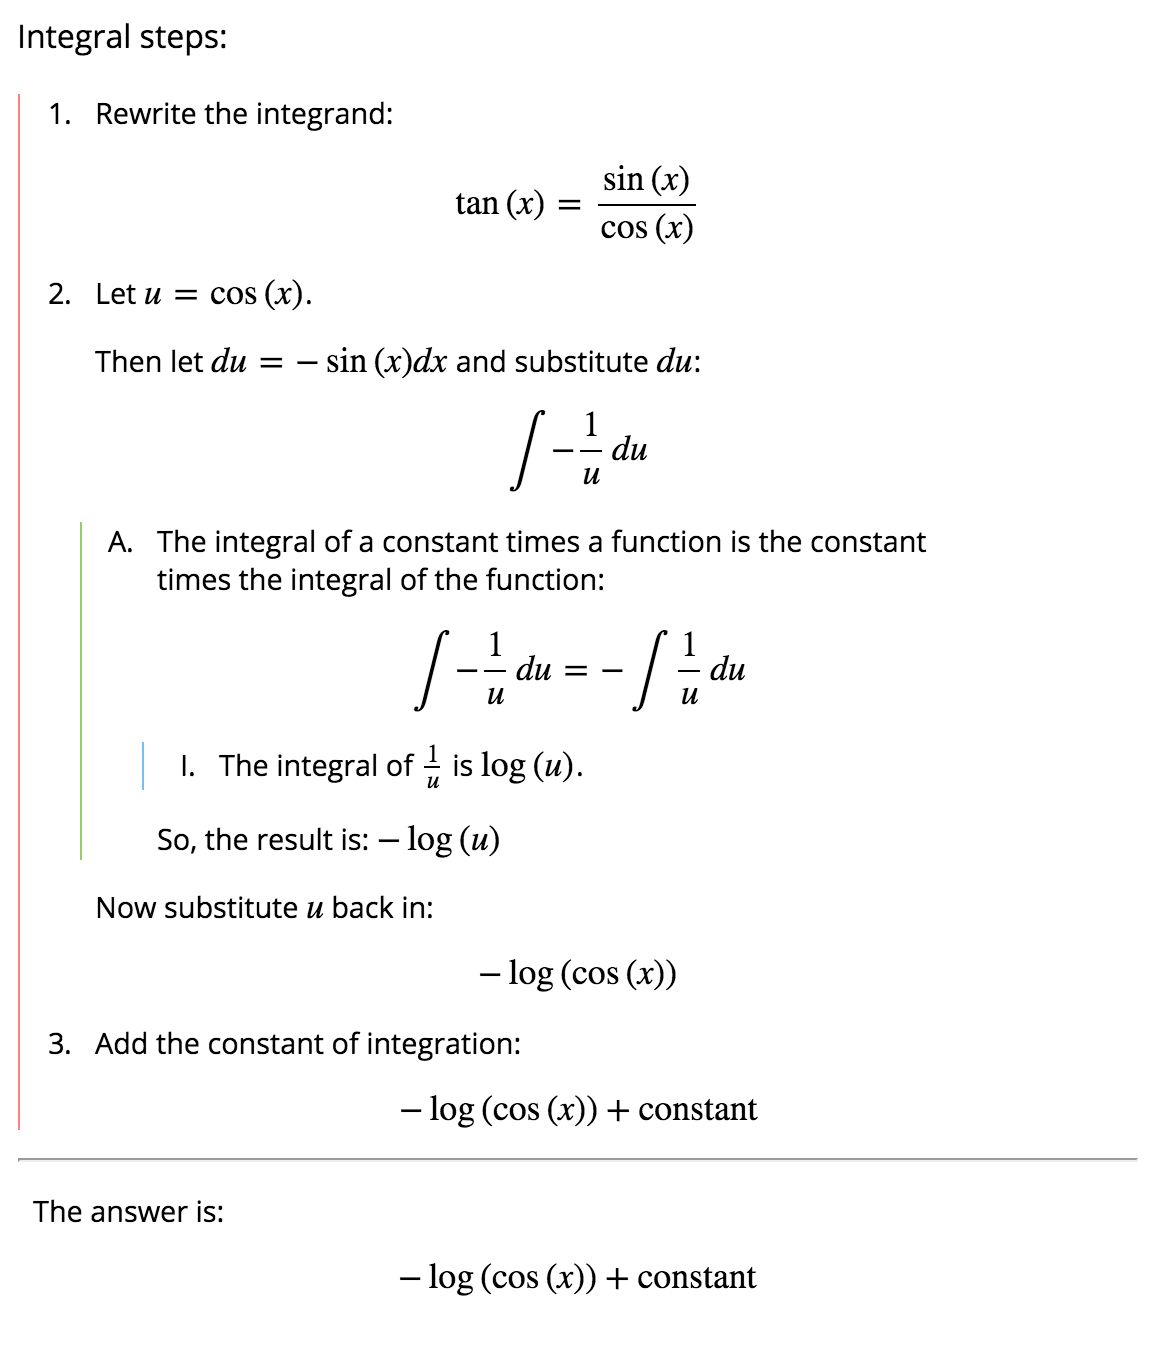
\includegraphics[width=0.7\textwidth]{supp-fig2-integral_steps.png}
    \captionof{figure}{\href{http://www.sympygamma.com/input/?i=integrate+tan\%28x\%29}{Integral steps of $\tan (x)$}.}\label{fig:integralsteps}
    \par
  }
\item
  SymPy Gamma displays the factor tree diagrams for different numbers.
\item
  SymPy Gamma saves user search queries.
\end{itemize}
Every input query from the user on SymPy Gamma is first parsed by its
own parser capable of handling several different forms of function names
which SymPy as a library does not support. For instance, SymPy Gamma
supports queries like \texttt{sin\ x}, whereas SymPy will only recognise
\verb|sin(x)|.

This parser converts the input query to the equivalent SymPy readable code,
which is then processed by SymPy, and the result is finally printed with the
built-in MathJax~\cite{cervone2012mathjax} output and rendered by the SymPy
Gamma web application.


\section{Comparison with Mathematica}
\label{suppsec:comp-mma}

Wolfram Mathematica is a popular proprietary CAS.\@
It features highly advanced algorithms.
Mathematica has a core implemented in C++~\cite{Wolfram2016}
which interprets its own programming language (know as Wolfram language).

% M-expressions

Analogously to Lisp's S-expressions,
Mathematica uses its own style of M-expressions,
which are arrays of either atoms or other M-expression.
The first element of the expression identifies the type of the expression
and is indexed by zero, whereas the first argument is indexed by one.
Notice that SymPy expression arguments are stored in a Python tuple
(that is, an immutable array),
while the expression type is identified by the type of the object storing the
expression.

% Attributes

Mathematica can associate attributes to its atoms.
Attributes may define mathematical properties and behavior of the nodes
associated to the atom.
In SymPy, the usage of static class fields is roughly similar to Mathematica's
attributes, though other programming patterns may also be used the achieve an
equivalent behavior, such as class inheritance.

% Expression mutability

Unlike SymPy, Mathematica's expressions are mutable,
that is one can change parts of the expression tree without the need of
creating a new object.
The reactivity of Mathematica allows for a lazy updating of any references
to that data structure.

% * comparison with Mathematica: commutativity, associative expressions, one-identity. Advantage of SymPy: multiplicative commutativity defined on symbols.
% Products and commutativity

Products in Mathematica are determined by some builtin node types,
such as \texttt{Times}, \texttt{Dot}, and others.
\texttt{Times} is overloaded by the * operator,
and is always meant to represent a commutative operator.
The other notable product is \texttt{Dot}, overloaded by the \texttt{.} operator.
This product represents matrix multiplication,
it is not commutative.
SymPy uses the same node for both scalar and matrix multiplication,
the only exception being with abstract matrix symbols.
Unlike Mathematica, SymPy determines commutativity with respect to
multiplication from the factor's expression type.
Mathematica puts the \texttt{Orderless} attribute on the expression
type.

% Associative expressions.

Regarding associative expressions,
SymPy handles associativity by making associative expressions inherit the
class \texttt{AssocOp},
while Mathematica specifies the \texttt{Flat}\cite{WolframRefFlat} attribute on the expression type.

% One identity


% Pattern matching

Mathematica relies heavily on pattern matching:
even the so-called equivalent of function declaration is in reality
the definition of a pattern matching generating an expression tree transformation
on input expressions.
%
Mathematica's pattern matching is sensitive to associative\cite{WolframRefFlat}, commutative\cite{WolframRefOrderless},
and one-identity\cite{WolframRefOneIdentity} properties of its expression tree nodes\cite{WolframRefFlatAndOrderlessFunctions}.
%
SymPy has various ways to perform pattern matching.
All of them play a lesser role in the CAS than in Mathematica
and are basically available as a tool to rewrite expressions.
The differential equation solver in SymPy somewhat relies on pattern matching to
identify the kind of differential equation, but it is envisaged to replace
that strategy with analysis of Lie symmetries in the future.
Mathematica's real advantage is the ability to add new overloading to the
expression builder at runtime, or for specific subnodes.
Consider for example
\begin{verbatim}
In[1]:= Unprotect[Plus]

Out[1]= {Plus}

In[2]:= Sin[x_]^2 + Cos[y_]^2 := 1

In[3]:= x + Sin[t]^2 + y + Cos[t]^2

Out[3]= 1 + x + y
\end{verbatim}
This expression in Mathematica defines a substitution rule that overloads
the functionality of the \texttt{Plus} node (the node for additions in Mathematica).
The trailing underscore after a symbol means that it is to be considered a
wildcard.
This example may not be practical, one may wish to keep this identity
unevaluated, nevertheless it clearly illustrates the potentiality to define
one's own immediate transformation rules.
In SymPy the operations constructing the addition node in the expression tree
are Python class constructors,
and cannot be modified at runtime.\footnote{In reality, Python supports monkey patching,
nonetheless it is a discouraged programming pattern.}
The way SymPy deals with extending the missing runtime overloadability functionality
is by subclassing the node types.
Subclasses may overload the class constructor to yield the proper
extended functionality.


%% TODO list:
% * comparison with Mathematica: MatrixExp, product not always commutative, type inheritance (polymorphism) and advantage in unifying the product symbol * for symbols and matrices, pattern matching vs. single dispatch.

% Type inheritance and polymorphism

Unlike SymPy, Mathematica does not support type inheritance or polymorphism~\cite{Fateman1992}.
% cite examples of class inheritance in SymPy:
%
SymPy relies heavily on class inheritance, but for the most part,
class inheritance is used to make sure that SymPy objects inherit the proper
methods and implement the basic hashing system.
Associativity of expressions can be achieved by inheriting the class \texttt{AssocOp},
which may appear a more cumbersome operation than Mathematica's attribute setting.
%There are also cases where inheritance is used to extend the mathematical meaning of an expression.

% Matrices

Matrices in SymPy are types on their own.
In Mathematica, nested lists are interpreted as matrices whenever the sublists
have the same length.
The main difference to SymPy is that ordinary operators and functions
do not get generalized the same way as used in traditional mathematics.
Using the standard multiplication in Mathematica performs an elementwise
product, this is compatible with Mathematica's convention of commutativity of
\texttt{Times} nodes.
Matrix product is expressed by the \textit{dot} operator,
or the \texttt{Dot} node.
The same is true for the other operators, and even functions,
most notably calling the exponential function \texttt{Exp} on a matrix
returns an elementwise exponentiation of its elements.
The real matrix exponentiationl is available through the \texttt{MatrixExp}
function.

% * comparison with Mathematica: avoid misspelling variables through forced declaration (check that you can't do it in Mathematica).
% * evaluate=False vs HoldForm

Unevaluated expressions can be achieved in various ways,
most commonly with the \texttt{HoldForm} or \texttt{Hold} nodes,
that block the evaluation of subnodes by the parser.
Note that such a node cannot be expressed in Python, because of greedy evaluation.
Whenever needed in SymPy, it is necessary to add the parameter \texttt{evaluate=False}
to all subnodes, or put the input expression in a string.

% * comparison with Mathematica: == is structural equality, not

The operator == returns a boolean whenever it is able to immediately evaluate
the truthness of the equality, otherwise it returns an \texttt{Equal} expression.
In SymPy == means structural equality and is always guaranteed to return a
boolean expression.
To express an equality in SymPy it is necessary to explicitly construct the
\texttt{Equality} class.

% * comparison with Mathematica: polynomial module.
% * comparison with Mathematica: space is product, ** vs ^

SymPy, in accordance with Python and unlike the usual programming convention,
uses ** to express the power operator, while Mathematica uses the more
common \verb|^|.

% * comparison with Mathematica: ( ) is Sequence, functions are generally uppercase.
% * comparsion with Mathematica: table of comparison?
% * comparison with Mathematica: Wolfram language has loads of operator overloading, functional paradigm.


\bibliography{paper}

\end{document}


\end{document}
